\documentclass[11pt,a4j]{jarticle}
\usepackage[dvipdfmx]{graphicx,color}
\usepackage{wrapfig}
\setlength{\topmargin}{-1.5cm}
\setlength{\textwidth}{15.5cm}
\setlength{\textheight}{25.2cm}
\newlength{\minitwocolumn}
\setlength{\minitwocolumn}{0.5\textwidth}
\addtolength{\minitwocolumn}{-\columnsep}
%\addtolength{\baselineskip}{-0.1\baselineskip}
%
\def\Mmaru#1{{\ooalign{\hfil#1\/\hfil\crcr
\raise.167ex\hbox{\mathhexbox 20D}}}}
%
\begin{document}
\newcommand{\fat}[1]{\mbox{\boldmath $#1$}}
\newcommand{\D}{\partial}
\newcommand{\w}{\omega}
\newcommand{\ga}{\alpha}
\newcommand{\gb}{\beta}
\newcommand{\gx}{\xi}
\newcommand{\gz}{\zeta}
\newcommand{\vhat}[1]{\hat{\fat{#1}}}
\newcommand{\spc}{\vspace{0.7\baselineskip}}
\newcommand{\halfspc}{\vspace{0.3\baselineskip}}
\bibliographystyle{unsrt}
\pagestyle{empty}
\newcommand{\twofig}[2]
 {
   \begin{figure}[h]
     \begin{minipage}[t]{\minitwocolumn}
         \begin{center}   #1
         \end{center}
     \end{minipage}
         \hspace{\columnsep}
     \begin{minipage}[t]{\minitwocolumn}
         \begin{center} #2
         \end{center}
     \end{minipage}
   \end{figure}
 }
%%%%%%%%%%%%%%%%%%%%%%%%%%%%%%%%%
%\vspace*{\baselineskip}
\begin{center}
{\Large \bf 令和1年度 共同研究報告書}
\end{center}
\vspace{2mm}
\begin{center}
{\LARGE \bf 結晶質岩を対象とした連成現象が\\
長期挙動におよぼす影響に関する研究} 
\end{center}
\begin{center}
岡山大学環境生命科学研究科\\
木本和志, 市川康明
\end{center}
\vspace{10mm}
%%%%%%%%%%%%%%%%%%%%%%%%%%%%%%%%%%%%%%%%%%%%%%%%%%%%%%%%%%%%%%%%
\section{はじめに}
%結晶質岩中のマイクロクラックは、岩盤の長期的な物質輸送特性や力学的な挙動に影響を与えると
考えられる。マイクロクラックの多くは肉眼で直接観測することは難しく、薄片を作成し偏光顕微鏡で
観察するなどして調べる必要がある。このような検査は非常に労力を要する上、
検査対象となる岩の状態をその場で非破壊的に調べる際には利用できない。
そのため、その場かつ非破壊的にマイクロクラックの状態を調べる技術があれば、
岩盤の現在の状態や長期の将来的な挙動を予想する上で有用な情報を提供刷ることができる。
そのような観点のもと、著者らは、超音波を使った花崗岩コア供試体の音響的性質の評価に
取り組んで来た。その結果としてこれまでに、粗大な結晶粒を有する花崗岩であっても、
数cm程度の距離であれば、数mmスケールの超音波を透過させることができることを示した。
また、レーザードップラー振動計を用いて波動場を詳細に観測することで、
鉱物粒と弾性波の相互作用を可視化できること、試料の部位や状態に応じて表面波速度に
有意な変化が現れることも明らかにしてきた。
これら音速の変化は、波動場の可視化結果からマイクロクラックの状態を
反映したものと予想されるものの、き裂の存在によって岩石の音響的性質が変化することの
より確実な証拠を見出すことが課題として残されていた。
花崗岩では、造岩鉱物自体が異方性を持ち、き裂が存在せずとも、異方性や散乱による
弾性波の減衰が起きる。そのため、みかけの異方性や減衰が観測されることから、
き裂の影響であるとそのまま結論を導くことはできない。
一方で、き裂は、岩盤が受ける応力場に起因して発生や進展した場合、応力場に応じた
配向性を示すことや、特定の鉱物に集中して発生する可能性が予想される。
従って、き裂の発生や成長に伴う音響異方性の変化や、特定の鉱物種の周辺で
生じる特異な散乱、鉱物種の含有割合におうじた音響的性質の変化を観察することが
き裂と弾性波の相互作用を理解し、計測波形からき裂の状態を推定する上で必要となる。
そのためには、鉱物粒からコアサンプルのスケールまで種々の空間解像度で弾性波散乱や
音響異方性を調べる方法が必要となる。
従来、岩石コアの音響的性質の評価では、圧電トランスデューサでコアサンプルを
透過した波動を計測しその音速や異方性を調べることが行われてきた。
この方法では、コア全体の平均的な性質は調べることができるものの、コアの部位や
鉱物の分布状況に応じてた音響的な性質の評価は行うことができない。
また、超音波を透過させることのできる方向は供試体の形状によって決まるため、
状況によっては、透過波を計測ができない方向もあり、音響異方性を調べることができない
場合もある。このことから、クラックの状態を知るための弾性波計測は、
供試体表面の任意の位置と方向で実施可能な方法を用いることが望ましい。
本年度の研究では、そのような計測の実現に向け、同一表面において、任意の方向と伝播
距離で超音波の送信と受信と行う方法を提案し、音響異方性の評価に利用可能である
ことを示した。具体的には、コアサンプル中央の
20mm角の領域が示す音響異方性を超音波波形から推定し、マイクロクラックに起因した
直交異方性が観察できることを明らかにする。
以下では、新たに構築した超音波計測系と 実験に用いた花崗岩コア供試体について述べる。
特に、強い超音波を送信するために新たに導入した集束型接触探触子の仕様と
導入の意図を述べる。計測点の配置や波形収録に関する設定について示した後、
実際に構築した計測系で得た超音波波形を示す。
次に、超音波波形から岩石コア試料の音響的性質を得るために、行った
波形処理の方法とその結果得られた音速やピーク周波数を示す。
最後に、入射方向によるそれら音響的性質の変化を示し。花崗岩よく知られている通り、
直交異方性を示すことが、表面波計測結果からも示されること、さらに、
波形振幅と音速の相関から、異方性はき裂に起因したものであることが示唆されることを
述べ、まとめと今後の課題について述べる。

\section{超音波計測試験}
%--------------------
\begin{figure}[h]
	\begin{center}
	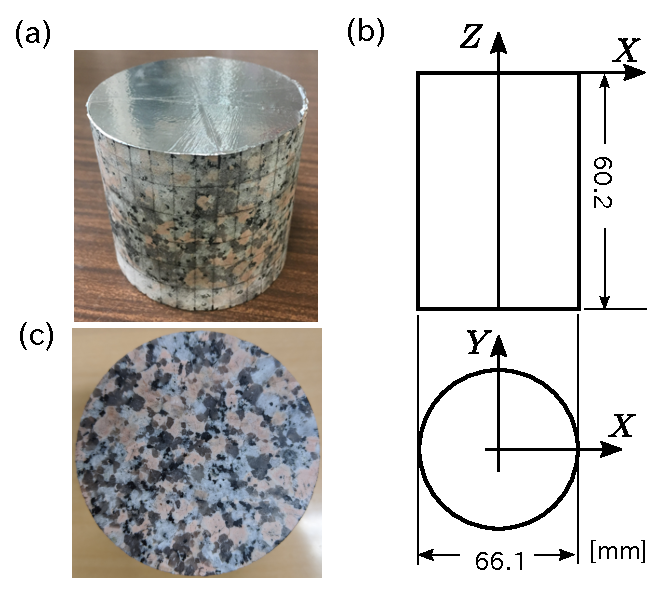
\includegraphics[width=0.6\linewidth]{Figs/fig1.eps} 
	\end{center}
	\caption{
		超音波計測に用いた花崗岩コア試料(万成花崗岩).
	} 
	\label{fig:fig1}
\end{figure}
%--------------------
%--------------------
\begin{figure}[h]
	\begin{center}
	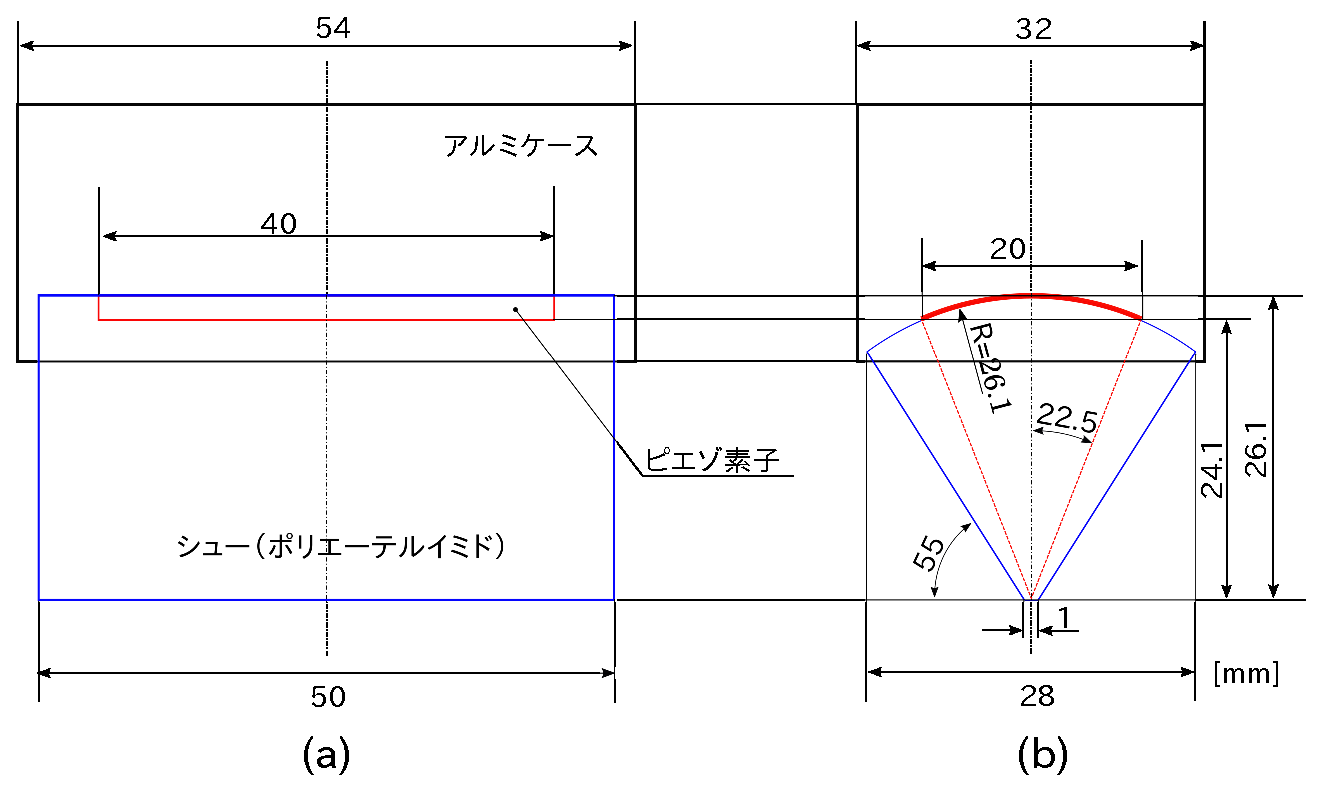
\includegraphics[width=0.8\linewidth]{Figs/fig2.eps} 
	\end{center}
	\caption{
		接触型ラインフォーカス探触子の形状と寸法.
	} 
	\label{fig:fig2}
\end{figure}
%--------------------
%--------------------
\begin{figure}[h]
	\begin{center}
	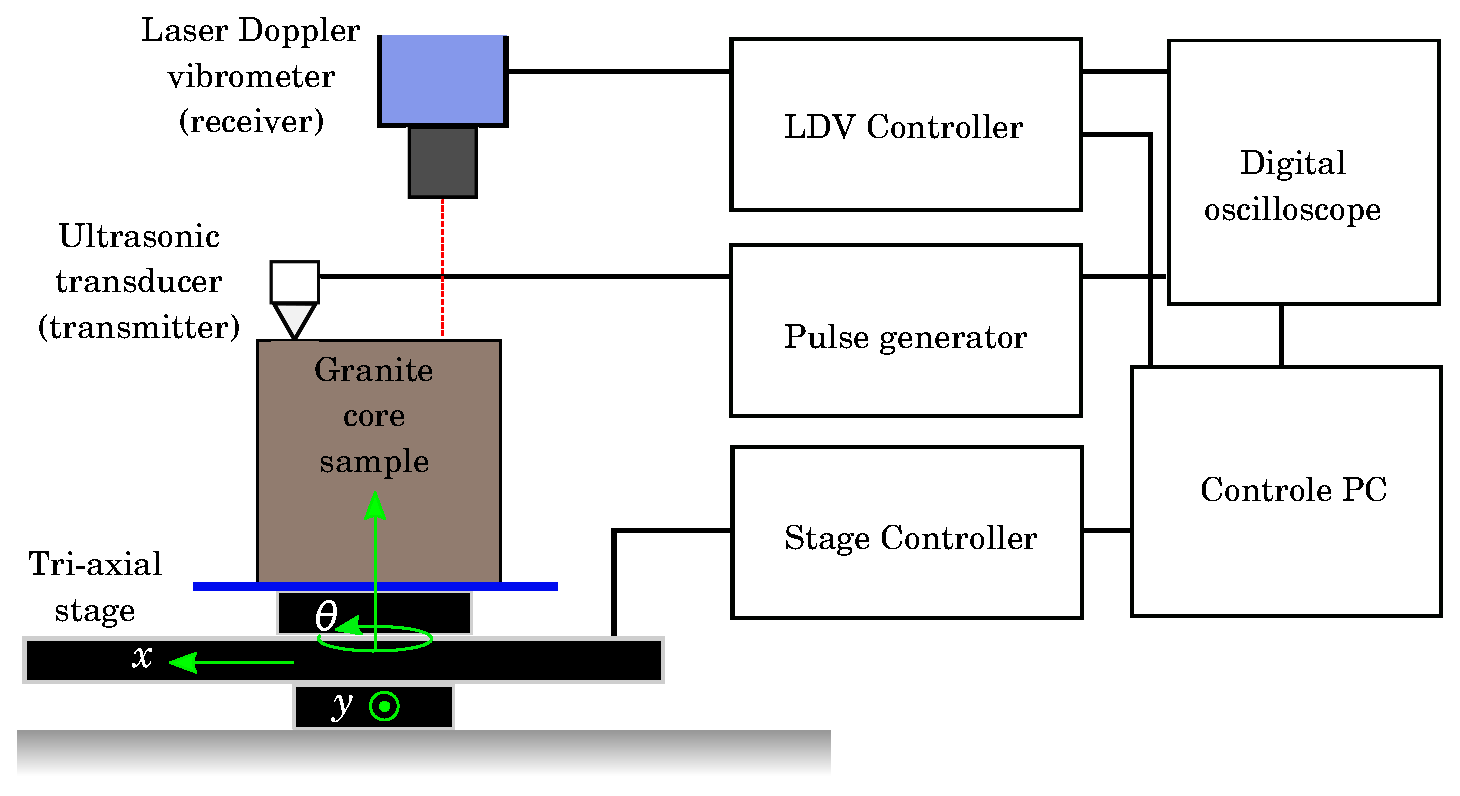
\includegraphics[width=0.8\linewidth]{Figs/fig3.eps} 
	\end{center}
	\caption{
		超音波測定装置の構成.
	} 
	\label{fig:fig3}
\end{figure}
%--------------------

\section{計測結果}
\subsection{送信波形の計測}
透過波形の計測に先立ち,入射波形に関する情報を得ることを目的として,
ラインフォーカス探触子先端部を供試体に接触させず,自由に振動させたときの
挙動を調べた.振動波形の取得にはLDVを用い,探触子の駆動は前節で述べた
条件によって行った.その結果得られた,探触子先端部の振動波形を図\ref{fig:fig5}に示す.
この図の(a)は振動速度の時刻歴を,(b)はその周波数スペクトルを示している.
時刻歴波形からは,シュー内部を超音波が伝播することによる時間遅れが
約11$\mu$secであることが読み取れる.また振幅値は,peak-to-peakで
およそ0.4V程度であることがわかる.これは,別途行った2.25MHz,
直径22.5mmの垂直接触型トランスデューサに比べ,約20倍程度大きな
振幅値で,圧電素子からの縦波がシュー先端部に集束し,強い超音波が励起
されていることを裏付けている.また,周波数スペクトルからは,周波数帯域
の上限が約3MHz,主たる周波数成分は1$\sim$2MHzにあることがわかる.
なお,シュー先端部で反射された波が,再度先端部に集束することも確認しているが,そ
の波形成分は30$\mu$sec付近にあり,時間軸上で完全に分離でき,以下で示す
計測の障害にはならない.
%--------------------
\begin{figure}[h]
	\begin{center}
	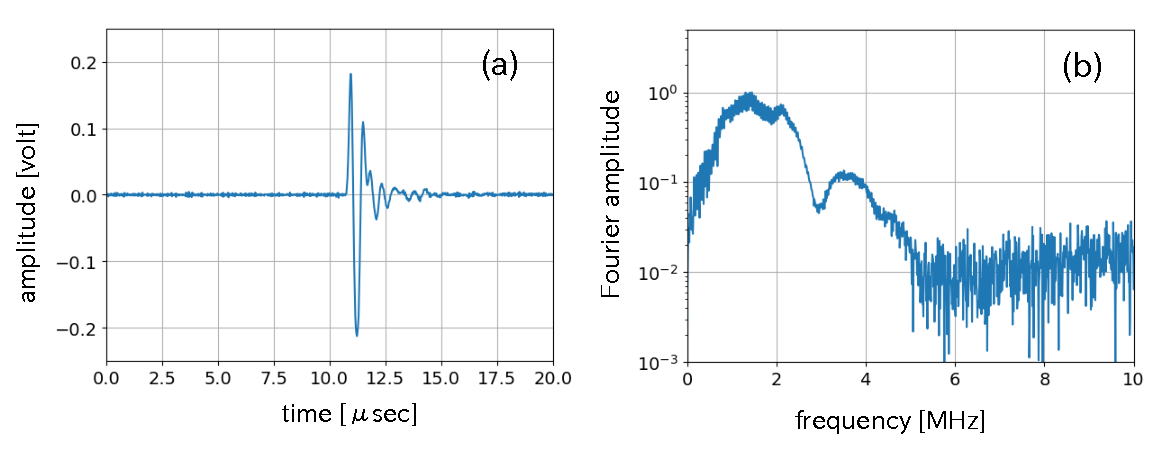
\includegraphics[width=0.9\linewidth]{Figs/fig5.eps} 
	\end{center}
	\caption{
		レーザードップラー振動計で計測したラインフォーカス探触子シュー先端部の振動速度波形.
	} 
	\label{fig:fig5}
\end{figure}
%--------------------
\subsection{透過波波形}
花崗岩コア供試体を用いて計測した,透過波の時刻歴波形を図\ref{fig:fig5_2}と\ref{fig:fig5_3}に示す.
これらの図には,入射方向の異なる6つの走時プロットを示している.
各々の走時プロットは,横軸が時間$t$($\mu$sec)を,縦軸は計測位置の$y$座標(mm)を表し,
$(t,y)$で観測された波形振幅をカラー表示している.
なお,波形振幅は,測線内で観測される最大振幅で無次元化している.
いずれの入射方向でも,19$\mu$sec前後に大きな振幅を持つ,位相の揃った表面波が到達し,その後,
多重散乱に起因したコーダ波が20$\mu$sec程度継続して観測されている.
位相の揃った初動成分の振幅は,場所によって大きな変動があり,波形も計測位置や入射方向に
よって異なることが分かる.このことから,個々の観測波形のピーク位置や到達時間から,
伝播速度を正確に求めることは困難であることが分かる.
そこで以下では,測線上で観測された波形データ全てを使い,平均的な表面波伝播速度を求める.
伝播速度は,群遅延から求めた群速度と,相互相関関数で評価した遅延時間から求めた
音速の2種類を入射方向毎に求め,供試体の音響異方性を調べる.
%--------------------
\begin{figure}[h]
	\begin{center}
	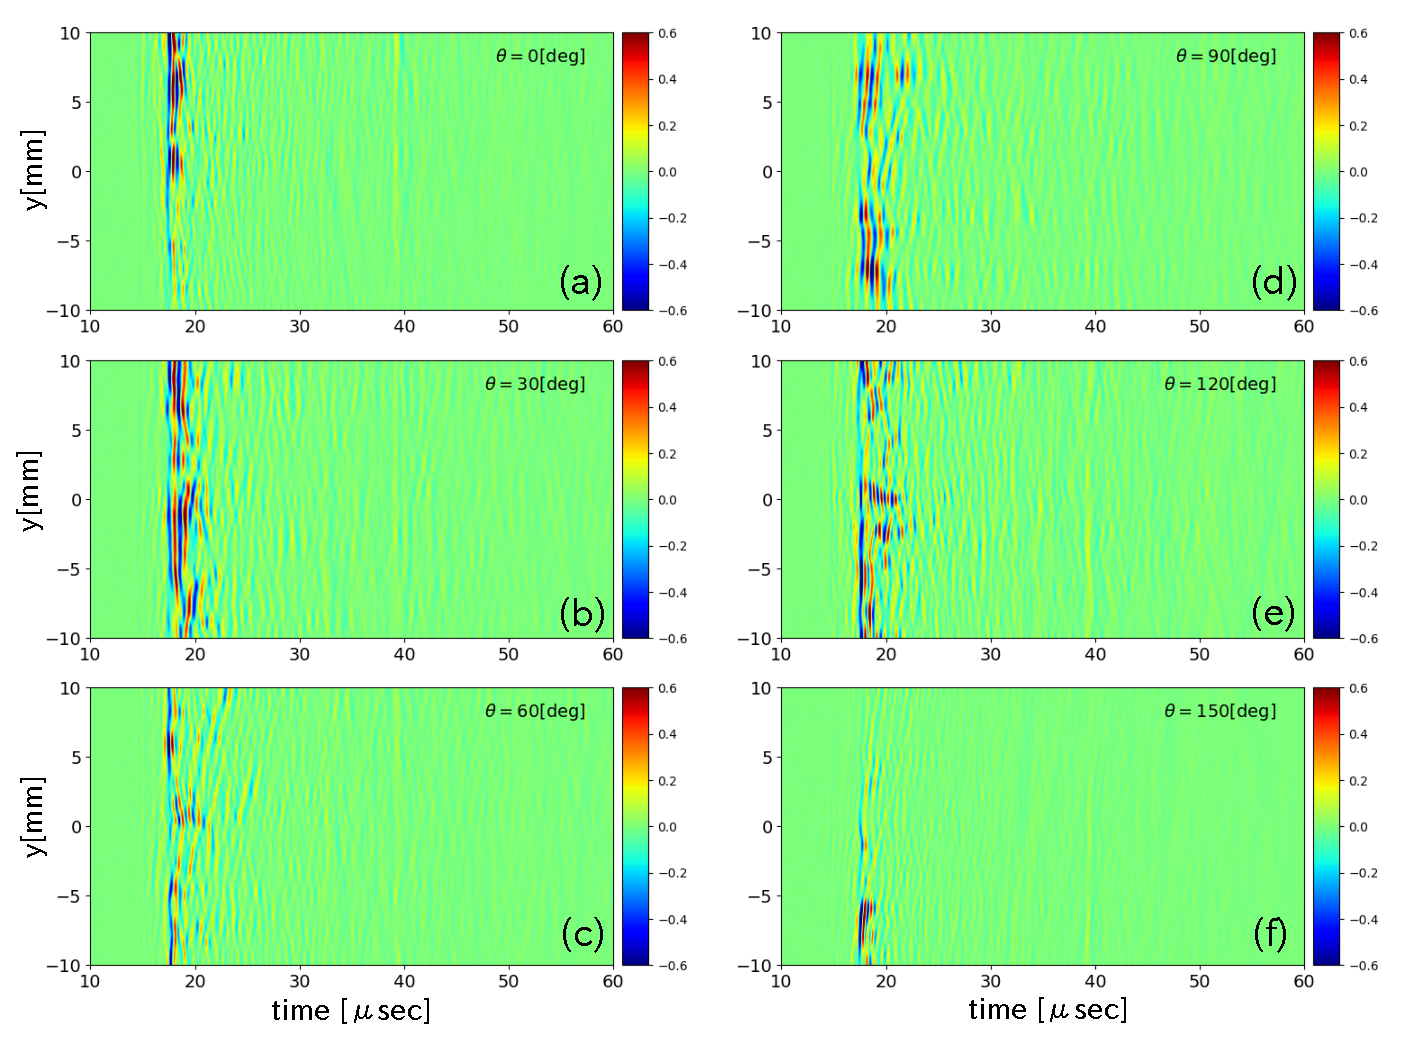
\includegraphics[width=1.0\linewidth]{Figs/fig5_2.eps} 
	\end{center}
	\caption{
		透過波波形の走時プロット(入射方向$\theta=0\sim 150^{\circ}$)
	} 
	\label{fig:fig5_2}
\end{figure}
%--------------------
\begin{figure}[h]
	\begin{center}
	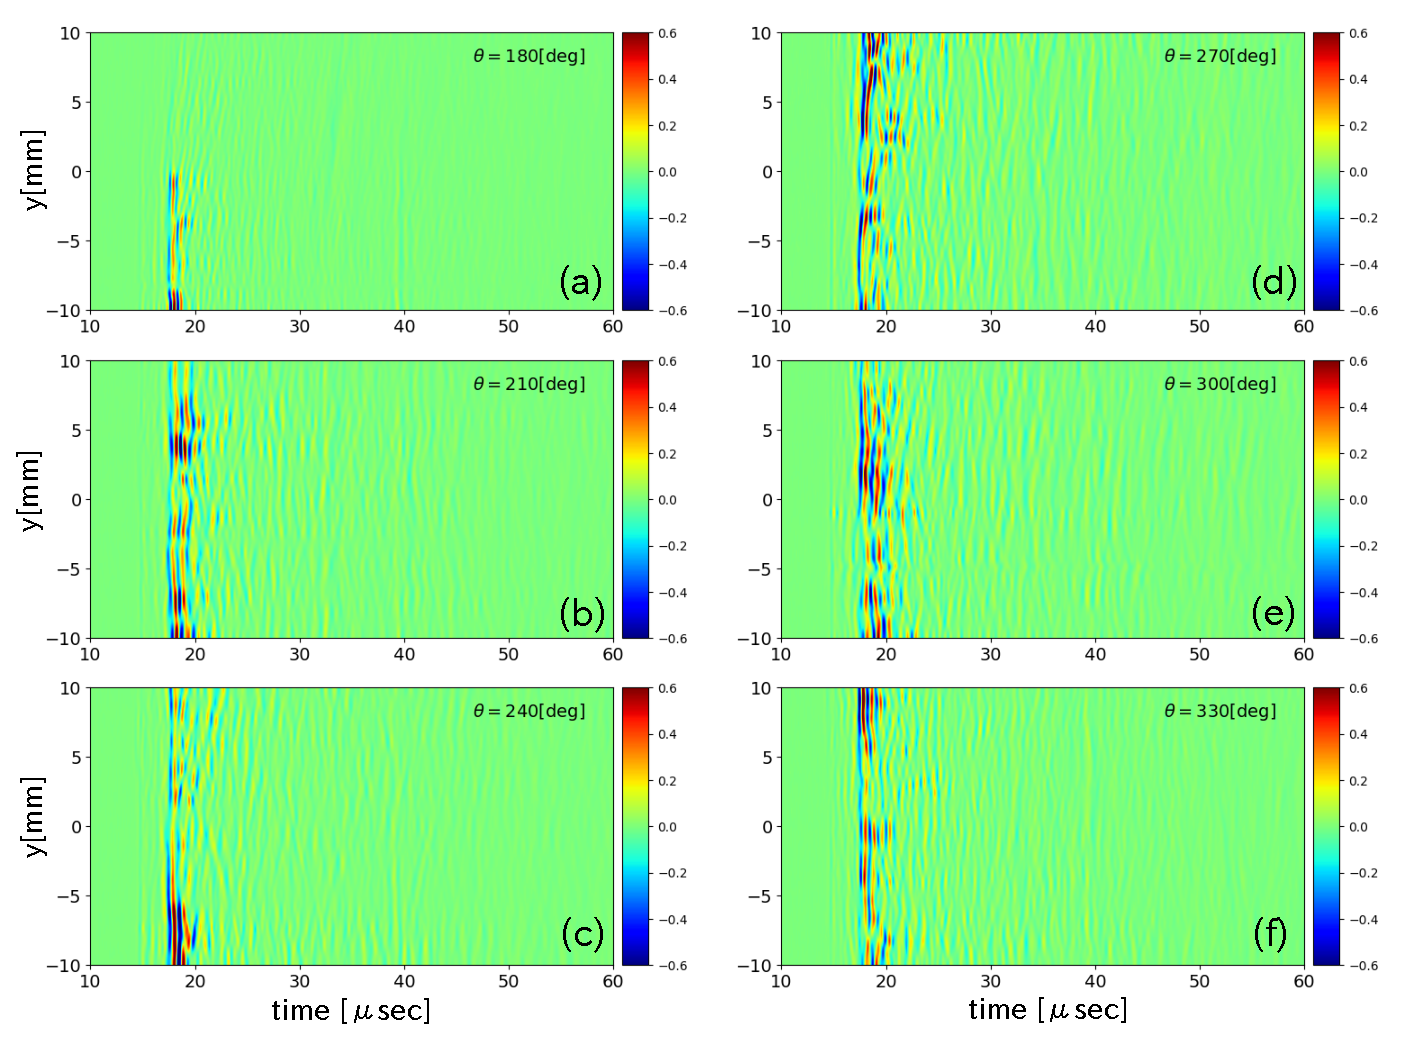
\includegraphics[width=1.0\linewidth]{Figs/fig5_3.eps} 
	\end{center}
	\caption{
		透過波波形の走時プロット(入射方向$\theta=180\sim 330^{\circ}$)
	} 
	\label{fig:fig5_3}
\end{figure}
%%%%%%%%%%%%%%%%%%%%%%%%%%%%%%%%%%%%%%%%%%%%%%%%%%%%%%%%%%%%%%%%%%%%%%
%%%%%%%%%%%%%%%%%%%%%%%%%%%%%%%%%%%%%%%%%%%%%%%%%%%%%%%%%%%%%%%%%%%%%%
\subsection{伝播速度の評価}
観測波形の初動成分を対象として伝播速度を評価するために,計測波形に時間軸上で
窓関数を作用させ,初動部近傍の大きな振幅を持つ波形部分を取り出す.
窓関数には,次式で与えられるButterworth関数を用いる.
\begin{equation}
	W(t;t_{1/2},m)=
	\left\{
		1+\left(\frac{t}{t_{1/2}}\right)^m
	\right\}^{-1}
	\label{eqn:Butterworth}
\end{equation}
Butterworth関数は,$m$が偶数のとき$t=0$について対称である.
その場合,$t_{1/2}$は振幅が半分となる時刻を,$m$は$t\rightarrow \pm \infty$
における減衰の速さを制御するパラメーターとして機能する.
ここで,$\cal R$上の位置$y$で観測される時間波形$a_{raw}(y,t)$とすれば,
Butterworth窓関数をかけて取り出された波形は
\begin{equation}
	a(y,t)=a_{raw}(y,t)W(t-t_b;t_{1/2},m)
\end{equation}
と表わされる.ここで,
\[
	t_b=18.2[\mu sec], \ \ t_{1/2}=2[\mu sec], \ \ m=6
\]
として観測波形に窓関数を作用させると,$\theta=0$[deg]では,図\ref{fig:fig6}の
ような結果が得られる.これを,図\ref{fig:fig5_2}-(a)を比べると,初動部分の
波形をほとんど変化させること無く,コーダ波が消去されていることが分かる.
次に,$a(y,t)$の時間に関するフーリエ変換を
\begin{equation}
	A(y, \omega)=\int a(y, t)e^{-i\omega t}dt=\left| A(\omega) \right|e^{i\phi}
	\label{eqn:def_FFT}
\end{equation}
を計算し,スペクトログラムとして表示すると,図\ref{fig:fig7}のようになる.
スペクトログラムからは,いずれの観測点位置における波形もおよそ3MHz程度までの
周波数成分が含まれており,入射波の持つ周波数成分を大きく損なうことなく,
岩石中を超音波が透過していることが分かる.
なお,図\ref{fig:fig6}に白の実線で示した時刻は,各観測点で得られた波形が
負の最大値を示す時刻を表している.一方,図\ref{fig:fig7}における白の実線は,
フーリエ振幅の最大値を与える周波数を示す.


岩石供試体中の弾性波の平均的な伝播挙動について調べるために,入射方向毎,すなわち測線毎に
平均波形を合成する.ここで,空間変数$y$に関する平均化作用素を
\begin{equation}
	\left< \cdot \right> := 
	\frac{1}{ \left| {\cal R} \right| }\int_{\cal R}\left( \cdot \right)dy
	\label{eqn:averaging}
\end{equation}
と表すことにすれば,波形データ${\cal D}$
\begin{equation}
	{\cal D}(\theta)=\left\{ a(y,t) \left| y\in {\cal R}, \, {\cal S}(\theta)\right.\right\}
	\label{eqn:}
\end{equation}
に対する平均波形は
\begin{equation}
	\left< a\right>(t)=
	\frac{1}{\left| {\cal R}\right|}\int_{\cal R}a(y,t)dy
	\label{eqn:def_mean_wv}
\end{equation}
で計算することができる.ただし,$\left| {\cal R }\right|$は,測線$\cal R$の長さ(20mm)を表す.
図\ref{fig:fig8}に,式(\ref{eqn:def_mean_wv})に従って計算した平均波形$\left<a \right>(t)$を
$\theta=0$[deg]の場合について,オレンジの実線で示す.この図には,ラインフォーカス探触子
のシュー先端部における自由振動波形$a^{ref}(t)$を参照波として青の実線で示している.
両者の振幅値は大きく異なることから,この図には二乗ノルムで正規化した結果を示している.
これらの波形の周波数スペクトルは,図\ref{fig:fig9}のようであり,透過波の平均波形は
参照波形と比べ2MHz以上の周波数成分が小さく,伝播の過程で相対的に高い周波成分が
多重散乱の結果,コーダ波に転じている.

平均的な伝播速度の評価には,群速度$c_g$と,計測波形と参照波形の相互相関関数から評価した速度を
$c_{cor}$を用いる.ここでは,後者を"相互相関速度"と呼ぶことにする.
各々の定義は以下のようである.
\paragraph{群速度}
波形$v(t)$のフーリエ変換を
\begin{equation}
	V(\omega)=\int v(t)e^{-i\omega t} dt = \left| V(\omega) \right|e^{i\phi(\omega)}
	\label{eqn:phase}
\end{equation}
とし,その,アンラップされた位相角を$\phi(\omega)$とする.このとき,波形$v(t)$の
群遅延$t_g(\omega)$は
\begin{equation}
	t_g(\omega)=-\frac{d\phi}{d\omega}
	\label{eqn:def_gdelay}
\end{equation}
で与えられる.
図\ref{fig:fig11}は,位相角$\phi(\omega)$を平均波形$\left<a\right>(t)$と参照波形$a^{ref}(t)$
について実際に計算したものである.両者とも周波数に対して直線的に変化しており
線形位相遅れでよく近似できることが分かる.そこで,式(\ref{eqn:def_gdelay})の微分を
位相角を直線で最小2乗近似したときの直線の勾配として評価する.
そのため,$t_g$は周波数依存性はなくなり,一つの波形に対して一つの群遅延が与えられることになる.
このような方法で求めた,観測波形と参照波形の群遅延をそれぞれ$t_g, t_g^{ref}$とし,
観測波の透過距離を$L$とすれば,群速度$c_g$は
\begin{equation}
	c_g=\frac{L}{t_g-t_g^{ref}}
	\label{eqn:def_cg}
\end{equation}
で与えられる.位置$y$で得られた波形について計算した群速度を$c_g(y)$とすれば,その$y$に関する
平均$\left< c_g \right>$を考えることができる.また,平均波形$\left<a\right>(t)$についても群速度を
求めることができ,この意味での平均群速度を $\bar c_g$と表す.
$\bar c_g$と$\left< c_g \right>$とも,入射方向毎に求めることができるため,
入射方向への依存性を明示する際には,それぞれ,$\bar c_g(\theta), \left< c_g\right>(\theta)$
と書くことにする.
\paragraph{相互相関速度}
参照波形$a^{ref}(t)$と観測波形$a(t)$の相互相関関数を
\begin{equation}
	{\rm Cor}\left(a,a^{ref}\right)(t)=
	\frac{
	\int a(\tau)a^{ref}(\tau-t) d\tau
	}{
		\left\| a(t)\right\|
		\left\| a^{ref}(t)\right\|
	}
	\label{eqn:def_Cor}
\end{equation}
で定義する.Cor$(a,a^{ref}(t)$のピークを与える時刻$t_{f}$,すなわち
\begin{equation}
	t_{f}:={\rm argmax} \left\{
		-{\rm Cor}\left(a,a^{ref}\right)(t)
		\right\}
	\label{eqn:def_tof}
\end{equation}
を波動の到達時刻と考えれば,透過波の伝播速度(相互相関速度)は
\begin{equation}
	c_{cor}=\frac{L}{t_{f}}
	\label{eqn:}
\end{equation}
で求めることができる.このようにして決定した相互相関速度についても空間平均と,
平均波形に対するものを考えることができる.それぞれ,群速度の場合と同様,
$\bar c_{cor}(\theta), \left< c_{cor}\right>(\theta)$
と書くこととする.
図\ref{fig:fig11}は,式(\ref{eqn:def_Cor})によって計算した相互相関関数を
示したものである.横軸は時間$t$を,縦軸は波形観測位置$y$を表し,観測点毎に得られる
相互相関関数値をカラー表示している.
図中の白の実線は,相互相関関数の負のピーク位置$t_{f}$を示している.
%--------------------
\begin{figure}[h]
	\begin{center}
	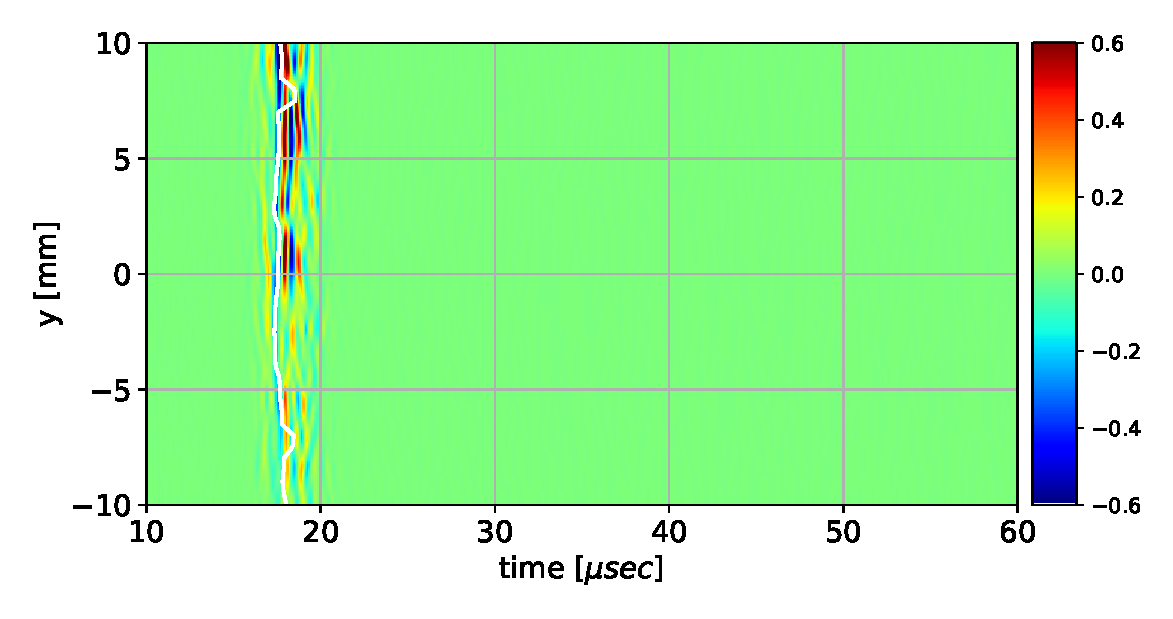
\includegraphics[width=0.7\linewidth]{Figs/fig6.eps} 
	\end{center}
	\caption{
		Butterworth窓関数で初動部分を取り出した結果の一例
		(入射方向$\theta=0^{\circ}$の場合)
	} 
	\label{fig:fig6}
\end{figure}
%--------------------
\begin{figure}[h]
	\begin{center}
	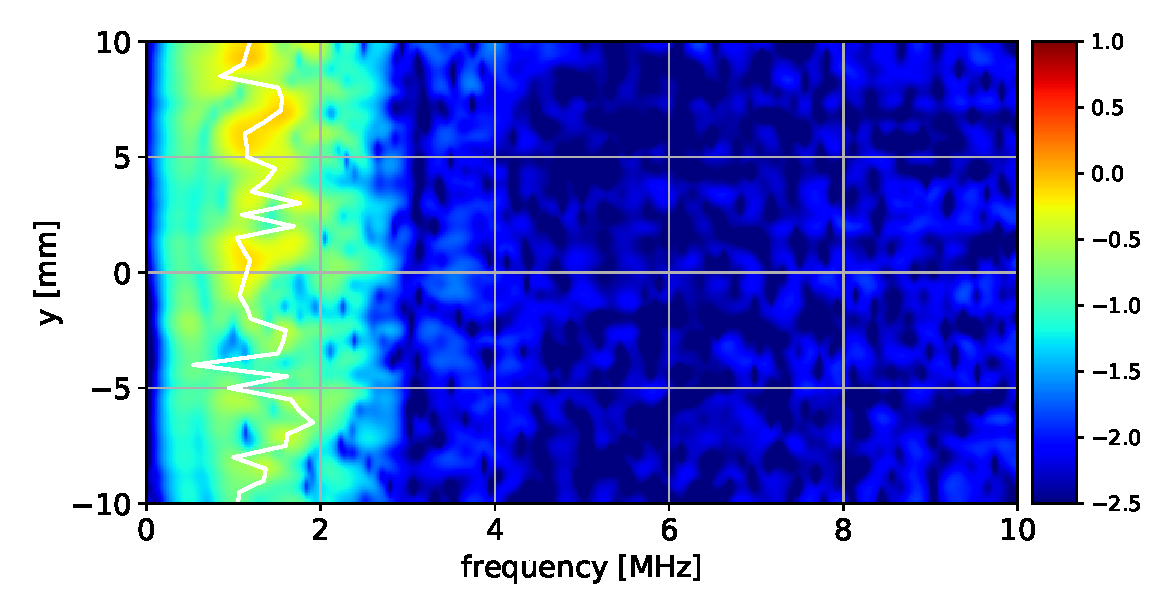
\includegraphics[width=0.7\linewidth]{Figs/fig7.eps} 
	\end{center}
	\caption{
		計測波形の初動部分に対する周波数スペクトログラム(入射方向$\theta=0^{\circ}$の場合).
	} 
	\label{fig:fig7}
\end{figure}
%--------------------
\begin{figure}[h]
	\begin{center}
	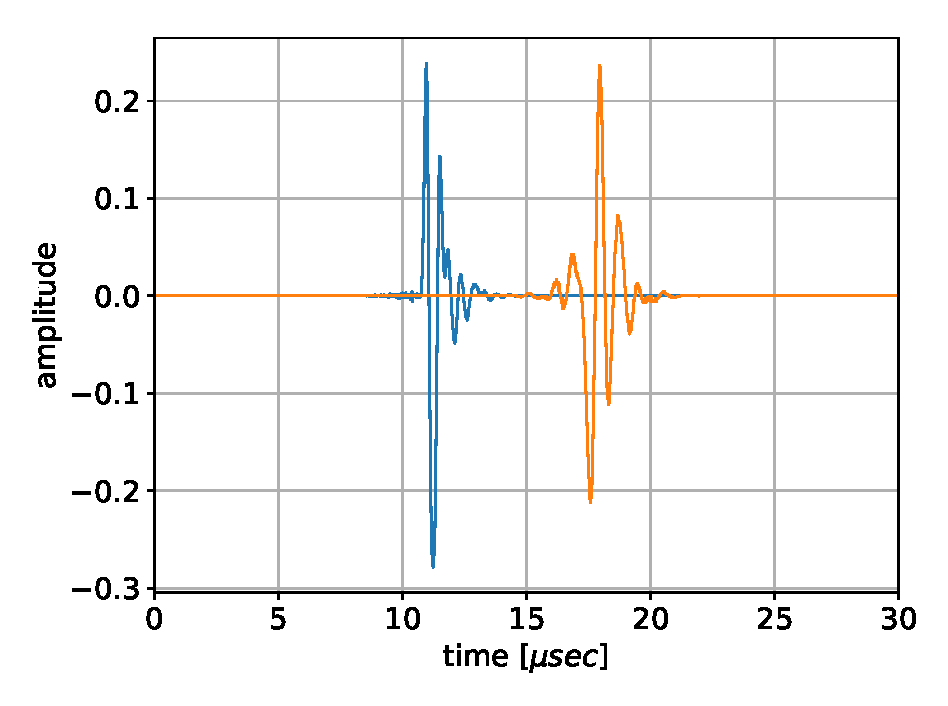
\includegraphics[width=0.6\linewidth]{Figs/fig8.eps} 
	\end{center}
	\caption{
		平均波形の時刻歴(オレンジの実線,入射方向$\theta=0^{\circ}$の場合).
		青はラインフォーカス探触子シュー先端部の自由振動波形に窓関数を
		作用させたものを参照波形として示す.
	} 
	\label{fig:fig8}
\end{figure}
%--------------------
\begin{figure}[h]
	\begin{center}
	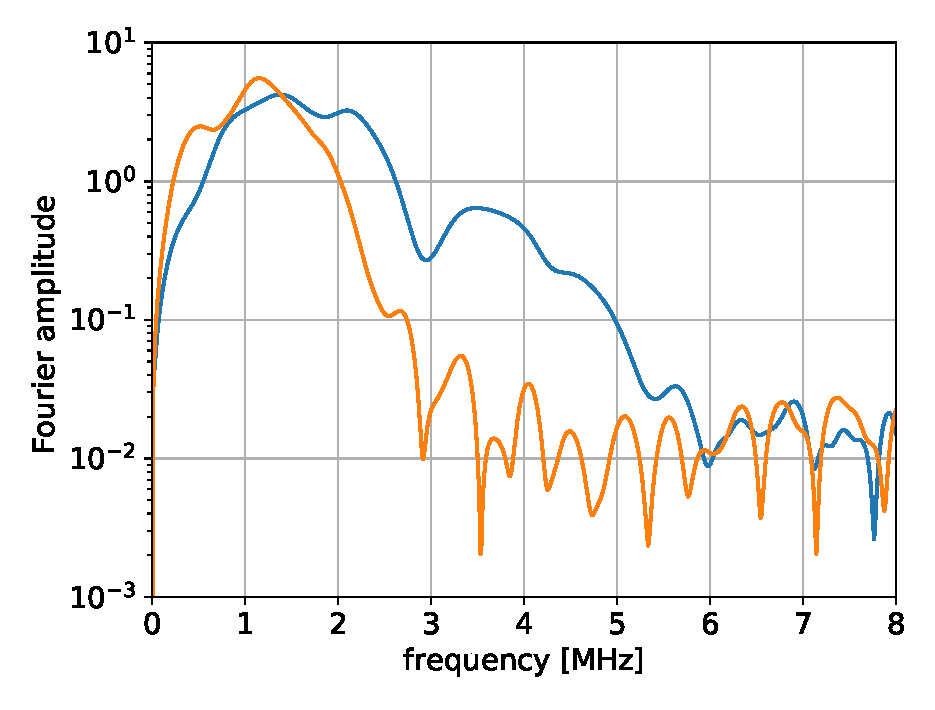
\includegraphics[width=0.6\linewidth]{Figs/fig9.eps} 
	\end{center}
	\caption{
		平均波形(オレンジ)と参照波形(青,シュー先端部の自由振動波形)の周波数スペクトル
		(入射方向$\theta=0^{\circ}の場合$).
	} 
	\label{fig:fig9}
\end{figure}
%--------------------
\begin{figure}[h]
	\begin{center}
	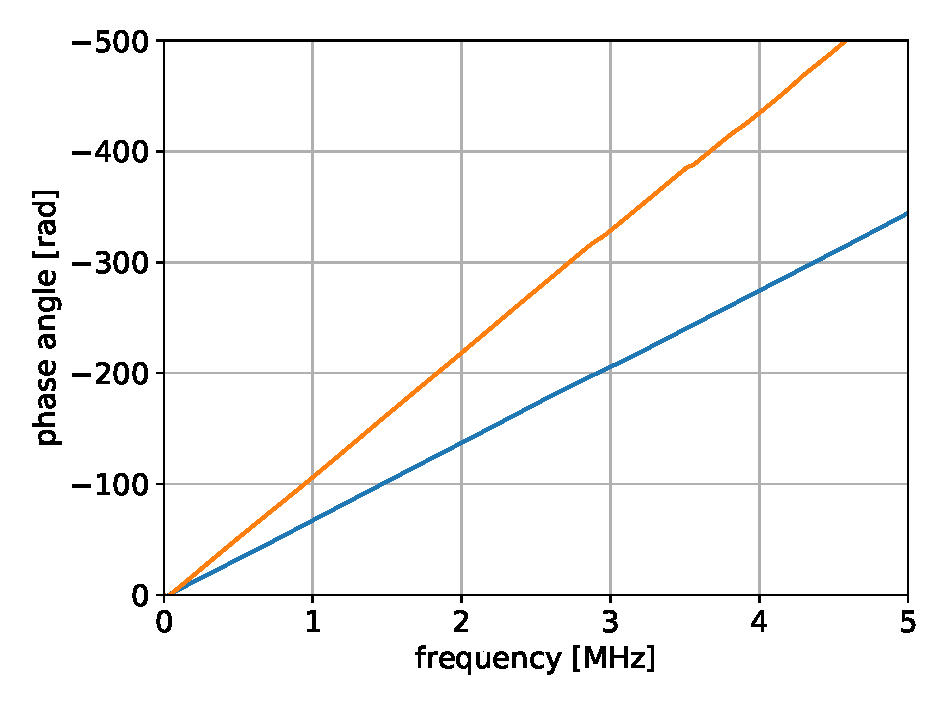
\includegraphics[width=0.7\linewidth]{Figs/fig10.eps} 
	\end{center}
	\caption{
		平均波形(オレンジ)と参照波形(青)の位相スペクトル(入射方向$\theta=0^{\circ}$の場合).
	} 
	\label{fig:fig10}
\end{figure}
%--------------------
\begin{figure}[h]
	\begin{center}
	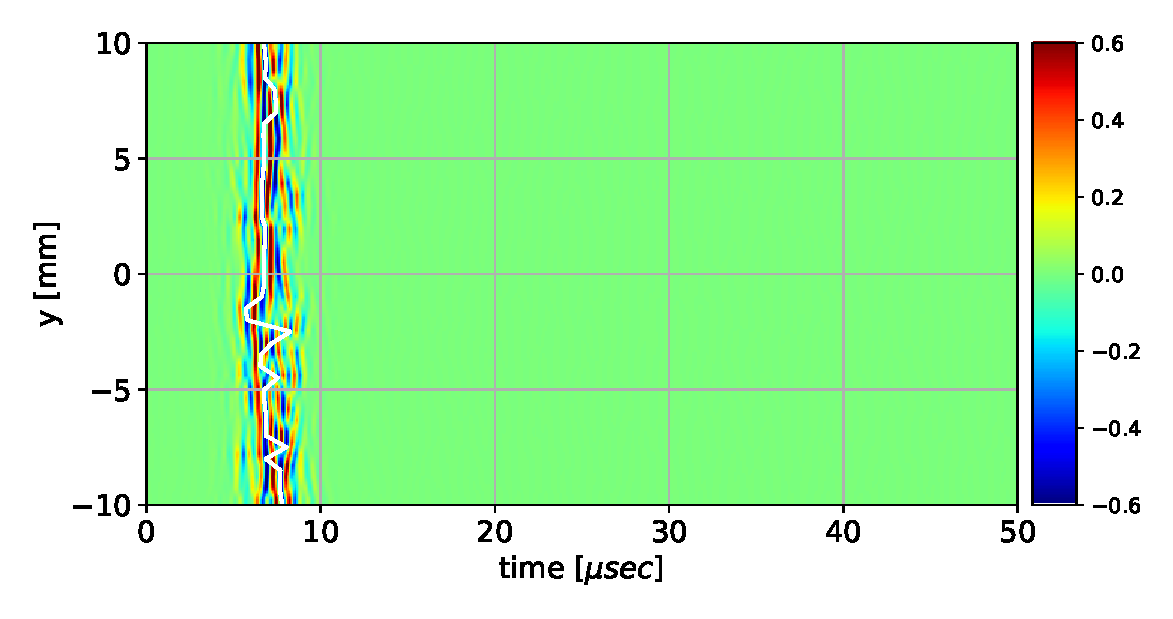
\includegraphics[width=0.7\linewidth]{Figs/fig11.eps} 
	\end{center}
	\caption{
		観測波形$a(y,t)$と参照波形$a^{ref}(t)$の時間に関する相互相関関数(入射方向$\theta=0^{\circ}$の場合).
	} 
	\label{fig:fig11}
\end{figure}
%--------------------


\section{速度および振幅変動分布の解析}
%各入射方向における測線で得られた波形データから群速度$\left<c_g\right>,\bar c_g$と
相互相関速度$\left<c_{cor}\right>, \bar c_{cor}$を計算した.その結果を
図\ref{fig:fig12}に示す.
この図は横軸が入射方向を,縦軸が音速値(km/s)を示している.
音速値は,概ね2.7(km/sec)から3.15(km/sec)の範囲にあり,主として表面波からなる
波動が観測されていることが分かる.この中で,最も方向による変化が大きいのは
平均群速度$\left<c_g\right>$で,$\theta=150$度と330度の方向で極大,
$\theta=30,240$度の方向で極小となっており,明確に音響異方性を示している.
一方,平均波形$\left<a \right>(t)$から求めた群速度$\bar c_g$の伝播方向による変動は
0.1(km/sec)と小さく,波形の平均化により速度の異方性が弱められることがわかる.
また,相互相関速度$\left<c_{cor}\right>$と$\bar{c}_{cor}$の挙動は,$\bar c_g$の挙動と
よく似ている.相互相関関数の計算では,参照波形として用いた入射波波形と類似した波形部分から到達時間を検出する.
そのため,最もよく位相が揃った波動が到達する時刻が得られるものの,観測点毎の速度変動が反映されにくいと考えられる.
以上のことから,音響異方性の評価には,局所的な群速度の平均$\left<c_g\right>$を見ることが
よいと言える.
%--------------------
\begin{figure}[h]
	\begin{center}
	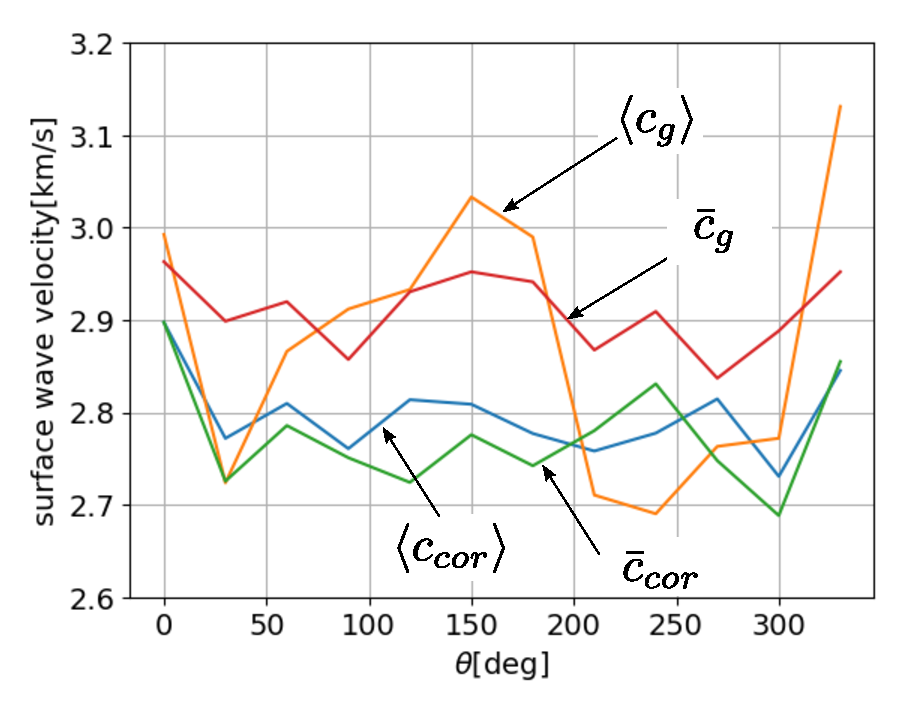
\includegraphics[width=0.8\linewidth]{Figs/fig12.eps} 
	\end{center}
	\caption{
		入射方向による群速度と相互相関速度の変化.
	} 
	\label{fig:fig12}
\end{figure}
%--------------------

ここで,入射方向毎に得られた平均波形$\left<a\right>(t)$を一覧すると,
図\ref{fig:fig11_1}のようになっている.
これら時刻歴波形の振幅はLDV出力の電圧値(mV)を表し,大小関係を波形相互に
比較でき,平均波形の最大振幅は明らかに方向によって変化している.そこで,
平均波形の最大振幅max$\left\{ \left< a \right>\right\}$と,
最大振幅の平均$\left< {\rm max}\left\{ a \right\} \right>$
が入射方向によってどのように変化するかを調べると,
図\ref{fig:fig14}のようになる.
この結果を図\ref{fig:fig12}と比べると,最大振幅の平均
$\left<{\rm max}\left\{a\right\}\right>$
は,$\left<c_g\right>$を上下に反転させたような形となり,強い異方性を
示すことが分かる.これは,群速度の速い方向で振幅が「小さく,
遅い方向で振幅が大きくなることを意味する.群速度と振幅値がこのような
相関を示すことは,岩石供試体の見かけの剛性が30度と240度方向で小さく,
150度と0度方向で大きくなるためと考えれば矛盾がない.
なお,平均波形の最大振幅max$\left\{\left<a\right>\right\}$は
最大振幅の平均よりも変動が若干小さい.これは,
波動到達時間の変動を考慮せずに最大値の平均をとる方が,
音響異方性をより敏感に反映した結果が得られることを意味する.
%--------------------
\begin{figure}[h]
	\begin{center}
	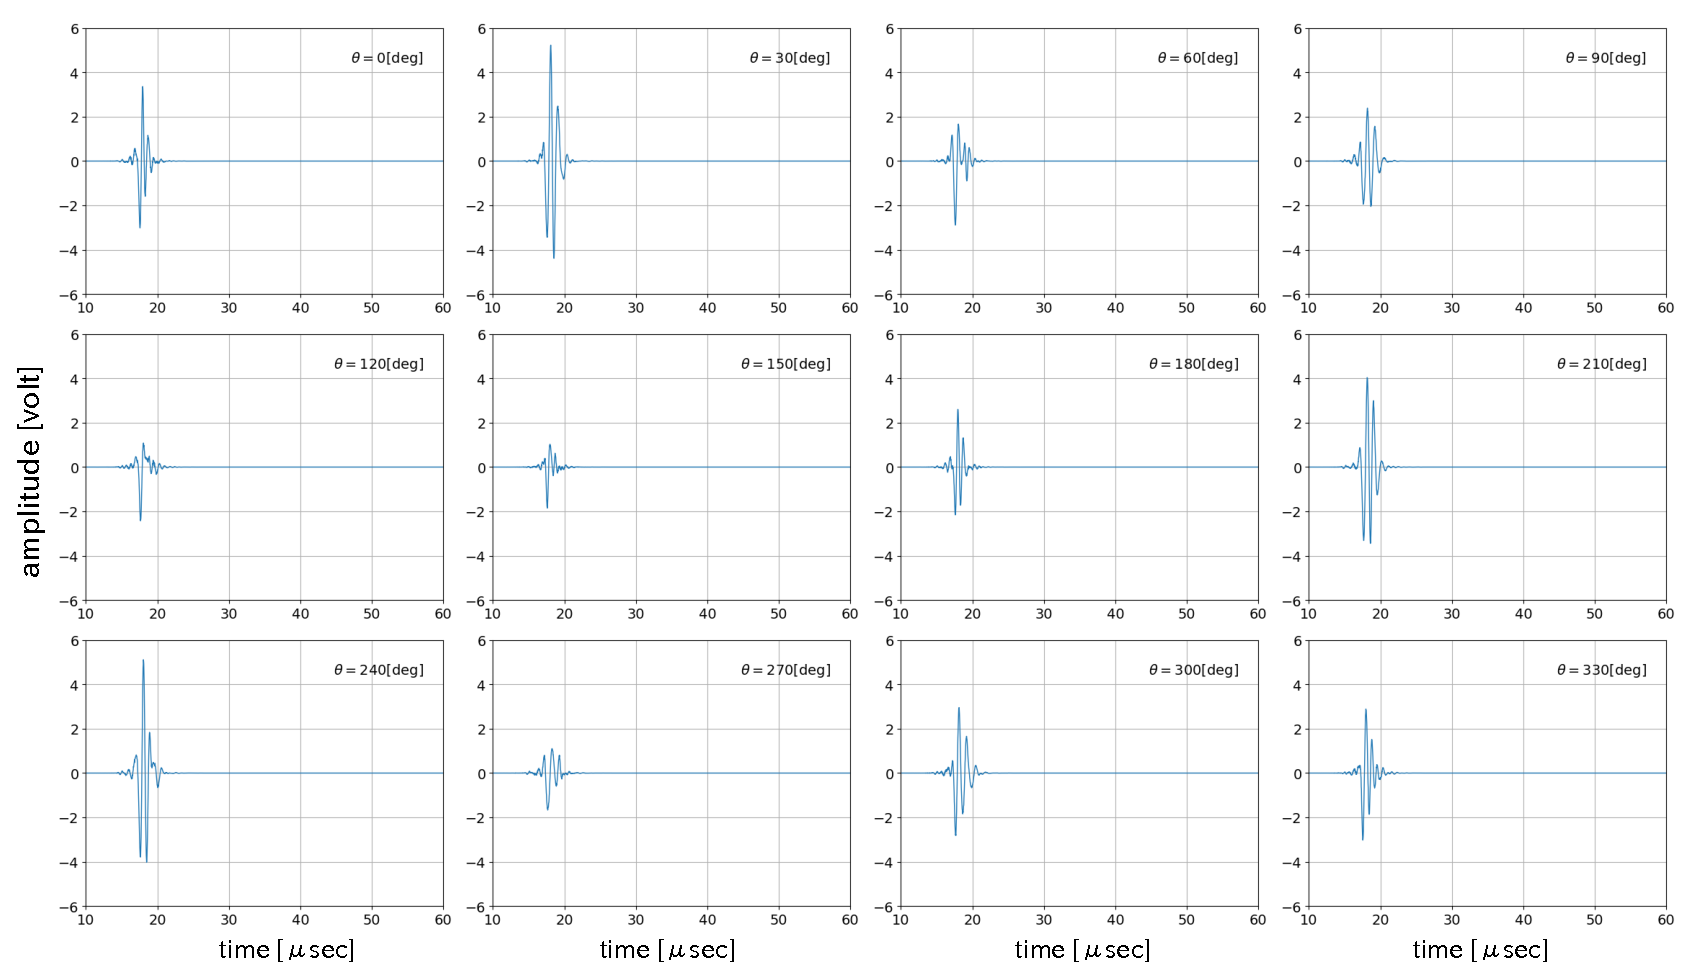
\includegraphics[width=1.0\linewidth]{Figs/fig11_1.eps} 
	\end{center}
	\caption{
		入射方向毎に得られた平均波形の時刻歴.
	} 
	\label{fig:fig11_1}
\end{figure}
%--------------------
\begin{figure}[h]
	\begin{center}
	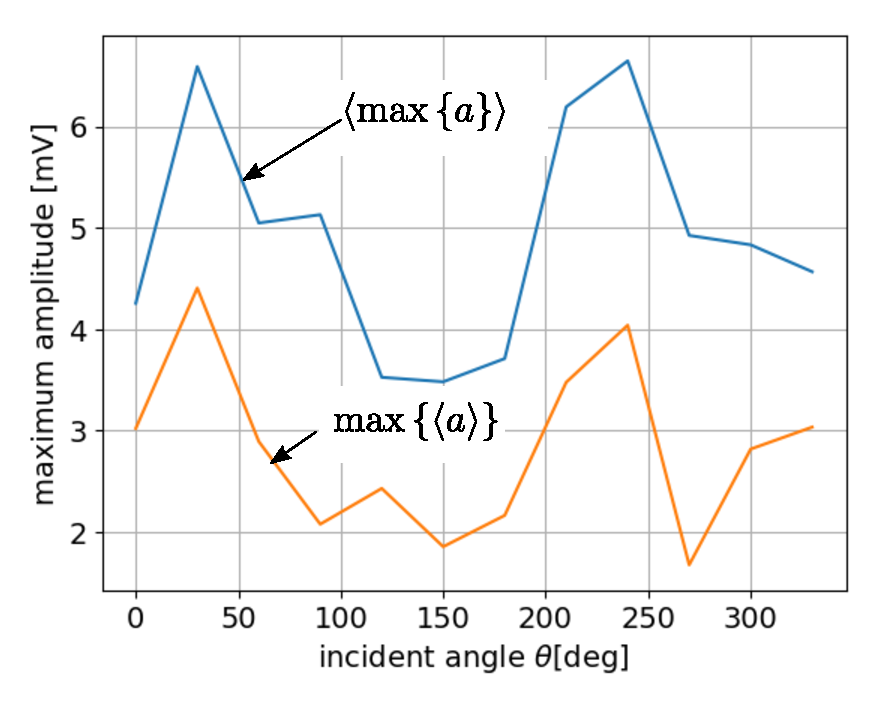
\includegraphics[width=0.8\linewidth]{Figs/fig14.eps} 
	\end{center}
	\caption{
		入射方向による最大振幅値の変化.
	} 
	\label{fig:fig14}
\end{figure}
最後に,平均波形の周波数スペクトル
\begin{equation}
	\left< A \right> (\omega) = \int \left<a\right>(t)e^{-i\omega t}dt
	\label{eqn:ave_A}
\end{equation}
を,入射方向毎に計算した結果を図\ref{fig:fig11_2}に示す.
これらの結果を見ると,周波数帯域はいずれの方向でも3MHz程度までとなっており,
その点に大きな違いは無い.一方,ピーク周波数には明らかなばらつきがあることに
気付く.そこで,平均波形のピーク周波数argmax$\left< A \right>$と,
個々の観測波形に対するピーク周波数の平均$\left< {\rm argmax }\left\{ A \right\}\right>$を求め,
角度との関係を示せば,図\ref{fig:fig13}のようになる.この図より,
ピーク周波数の平均$\left< {\rm argmax }\left\{ A \right\}\right>$は
$\left< c_g\right>$と似た傾向を示すことが分かる.具体的には,
群速度平均が大きな方向ではピーク周波数平均が高く,群速度平均が小さな方向では,
ピーク周波数平均は低くなっている.
これは,見かけの剛性が高い方が高周波の波を伝えやすく,みかけの剛性が低い方が
高周波成分を伝えにくいことを意味する.ここで,見かけの剛性と周波数が相関することは,
剛性の変化がマイクロクラックに起因したものであることを意味する.
なぜなら,線形弾性体では剛性の大小は振幅や音速に影響するが,周波数応答には
関与せず,剛性の周波数依存性は,界面の接触や滑りによってのみ生じるためである.
従って,ここで示した音響異方性に関する結果は,弾性波を使ったき裂評価において有用な
情報であると考えることができる.
なお,ピーク周波数の平均が,平均波形のピーク周波数よりも変動が小さい理由は
平均最大振幅と平均波形の最大振幅の大小に関する理由と同様である.
%--------------------
\begin{figure}[h]
	\begin{center}
	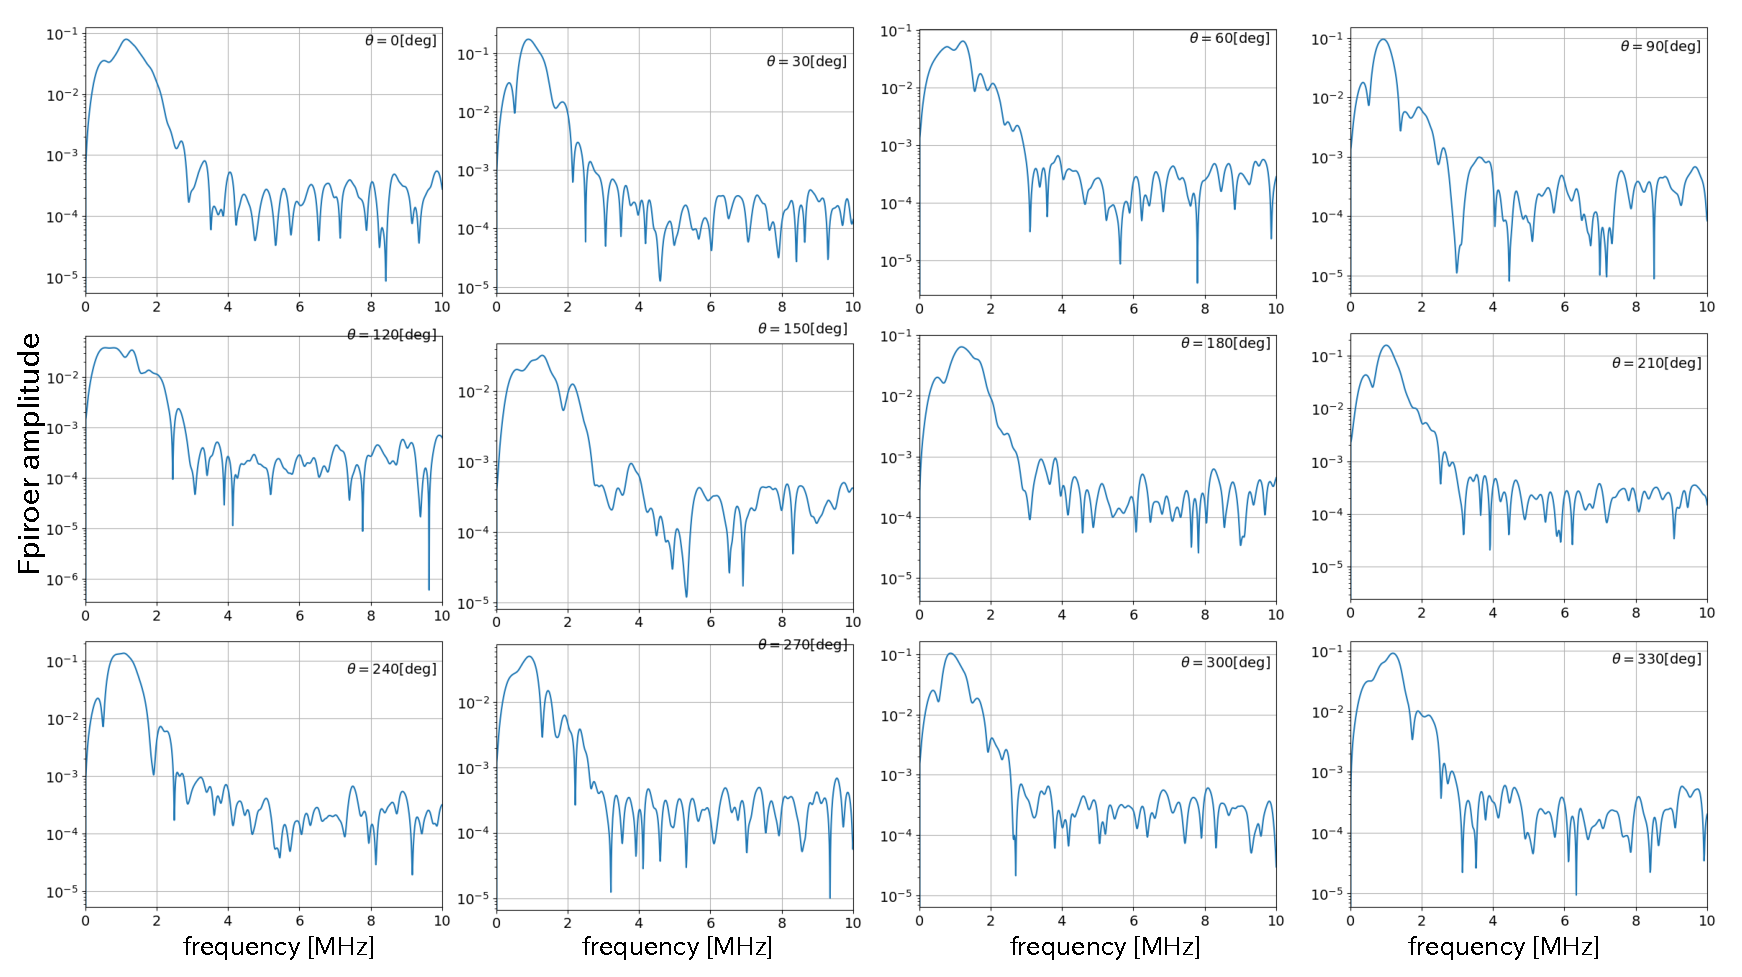
\includegraphics[width=1.0\linewidth]{Figs/fig11_2.eps} 
	\end{center}
	\caption{
		入射方向毎に得られた平均波形の周波数スペクトル.
	} 
	\label{fig:fig11_2}
\end{figure}
\begin{figure}[h]
	\begin{center}
	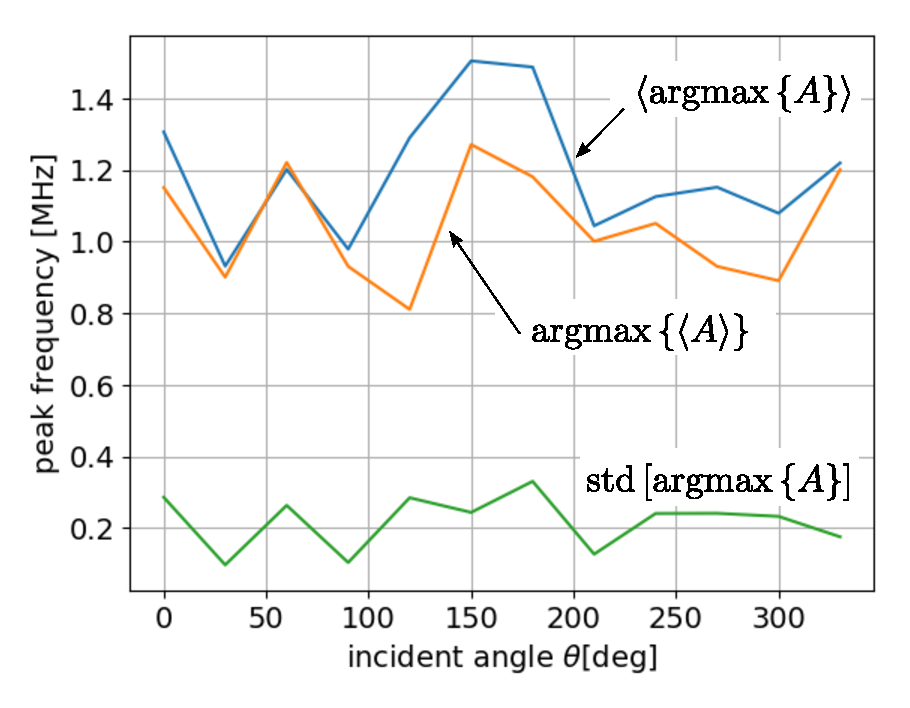
\includegraphics[width=0.8\linewidth]{Figs/fig13.eps} 
	\end{center}
	\caption{
		入射方向によるピーク周波の変化.
	} 
	\label{fig:fig13}
\end{figure}
%--------------------


%--------------------
\newpage
\section{まとめ}
本研究では,レーザードップラー振動計(LDV)を受信センサーとし,試料表面の
超音波振動を2次元的に走査して弾性波伝播挙動を可視化する自動計測システムの
構築を行った.ここで開発したシステムでは,指定された座標位置での弾性波計測
を順次自動的に行い,数千波形規模のデータセットを数時間から半日程度の所要時間
で取得することができる.これは,計測点間隔を0.5mmとした場合,50mm角程度の
正方形領域における波動伝播状況を可視化できることを意味する.
花崗岩は強い非均質のある多結晶質材料であるため,散乱波が発生直後の波形や指向性を
保ったまま伝播することが期待できない.また,散乱源となる音響的性質の
不均一性は至るところに存在することから,散乱波の発生や伝播状況に関する
情報を得るには,散乱源のごく近傍で,詳細な計測を行う必要がある.
花崗岩のような不均質材における波動伝播を十分な精度で再現できる理論モデルや
数値解析モデルは現時点では存在しないため,波動場の詳細を計測によって
明らかにすることは,今後,波動問題としての理論解析や数値解析を進める
際にも,モデリング上の仮定に根拠を与えるためや,モデルの精度評価を
行うために欠かせない情報を提供することができる.
そのような計測は,超音波非破壊検査の分野で広く用いられる圧電トランスデューサ
では実現が難しく,本研究のようにLDVを始めとするレーザーによる非接触計測
が今のところ最も現実的な手法と言える.

本研究においてLDVによる2次元自動スキャン計測結果から得られたデータの有用性
に関して言えば,多数の波形を正確に計測することが可能となった結果,伝播距離
に応じた波動場の平均的動を解析が可能となった.このことは同時に,
局所的な波動場が平均的挙動からのどの程度乖離しているかを定量化できる
ことを意味する.このような観点から,本年度の研究では,各計測点での振幅と
初動到達時間に関する偏差指標を定義し,実際に計測した波形データから評価
を行った.その結果,主としてカリ長石からなる部分は,音響的に高剛性な媒体
として,石英部分は低剛性な媒体として超音波に応答することが明らかとなった.
石英とカリ長石は音響異方性のタイプは異なるものの,密度と弾性波速度には
互いに大きな違いはない.そのため,石英の部分で音速や剛性の低下は,
き裂や音響的に柔らかい介在物の存在が予想され,花崗岩試料の
損傷評価や波動伝播モデリングにおいて重要な意味を持つ結果が得られた
と考えられる.

今後は,鉱物や損傷状態との関連がより明確で,同時に音響的な不均質性
を高いコントラストで再構成できる指標関数を考案することが重要な
課題の一つとなる.そのような指標として具体的には,局所的な弾性波速度
を用いることが考えられる.過去の研究では,試料全体での平均的な
群速度を求め,試料間で比較を行うといった検討は行ってきたが,
局所速度の評価と空間変動に関する検討は,十分な質と量の波形データ
取得が難しくこれまで実施していない.
局所速度を速度異方性と鉱物種との対応と併せて取得することができれば,
試料の性状評価や,弾性波モデリングに有用な多くの知見を提供することが
できると思われる.今回開発したLDV計測システムはその効果的な手段になると
期待される.一方,計測手法の開発に関する課題としては,送受信条件と
センサー仕様を最適化し,透過距離の影響を受けにくい形で試料の局所的
応答を計測する方法を開発することがが挙げられる.花崗岩は散乱減衰の
強い材料であるため,計測結果は入射波,散乱波とも伝播距離に影響を
受けやすい.とりわけ,高い周波数成分は散乱源のごく限られた範囲でしか
観測できない.これまでの計測では,1MHZ以上の周波数成分の挙動はほとんど
調べることができていない.しかしながら,高周波成分は試料の局所的な
状態に対して敏感に反応すると予想されることから,その計測と特徴の理解は,
花崗岩中の波動伝播挙動や不均質部との相互作用の理解を進める上で
大きな貢献につながると考えられる.
\end{document}
